\pattern{Template}
\begin{summary}
    Describes (and realizes) the common interactions between components. The
    {\bf template} pattern defines the skeleton of an algorithm for an
    operation while deferring some behaviour to the elements that are being
    operated on.
\end{summary}

Implementation details: \begin{itemize}
    \item Create a notion of an interface (either an interface or class) or
        a component of an algorithm that doesn’t vary between different
        datatypes (or both). Then use inheritance to create a specific
        implementation for the datatype addressed.
    \item in higher level languages (C\#, Java by type-erasure) where
        every class is a ``subclass'' of a super base class, (java.lang.Object
        in the case of Java), this can be used with many standard library
        algorithms and data structures
\end{itemize}

\comparison{\begin{itemize}
        \item ease of use: Creating a subclass based on the base class is easy
            to manage, it only requires the subclass to provide either a
            concrete implementation of an abstract method, or a more specific
            implementation of a method that is allowed by the base class.
        \item open-closed principle: The base class provides a
            framework that can be extended through inheritance to allow
            instances of new-but-related classes with new fields and methods.
            This allows designers to achieve new design requirements without
            having to change the code of the base class, or the algorithms and
            data structures which operate on instances of the base class.
        \item reusability: Code duplication is minimized through
            the use of base classes to establish a common pattern among
            subclasses. Subclasses only need to override methods that are not 
            defined for their use-case.
    \end{itemize}

}{\begin{itemize}
        \item flexibility: Due to its reliance on inheritance to establish the
            behavior of subclasses, usually subclasses are restricted to
            inheriting from one base class at a time. As a result, any subclass
            is restricted to follow the general behavior established by its
            parent base class.
        \item maintainability: Reading the flow of code is
            difficult due to the disjoint nature of the code. Code within the
            base class only provides the steps that its subclasses will take,
            whereas subclasses only contain details for a step. 
        \item tight coupling: Additional functionality is difficult to
            implement due to high coupling.  Adding features to the base class
            requires the change to be applied to all related subclasses.
    \end{itemize}
} % END of comparison

\begin{nfps}
\item[Something]
\end{nfps}

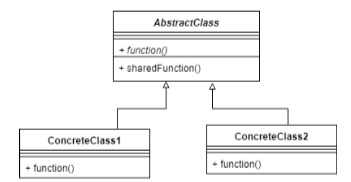
\includegraphics[width=0.5\textwidth]{./template1}
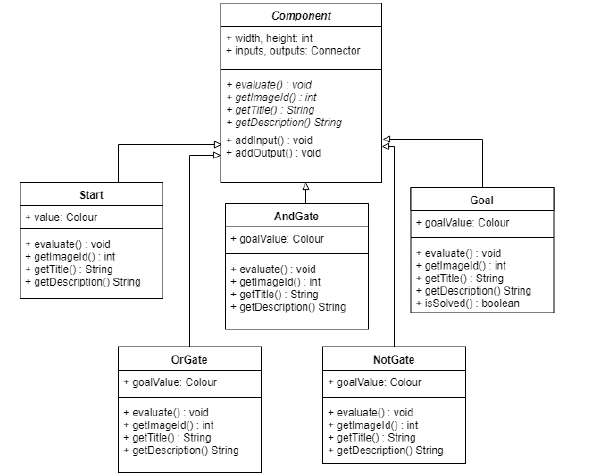
\includegraphics[width=0.5\textwidth]{./template2}
